\section{Efficient Enumeration of Ladder Lotteries and its Application}

%%Intro
In the Efficient Enumeration of Ladder Lotteries and its Application, written by Matsui, Nakada, Nakano Uehara and Yamanaka,
the authors provide an algorithm for generating $OptL\{\pi\}$ 
for any $\pi$, in $\mathcal{O}(1)$ per ladder~\cite{A1}. The authors refer to this algorithm as {\sc FindAllChildren}
which can be found in Algorithm~\ref{Alg:FindAllChildren}. 
\begin{algorithm}[!htp]
	\begin{algorithmic}[1]
		\Function{FindAllChildren}{$ladder$, $cleanLevel$, $n$}
			\State $currentRoute \gets n$
			\While{$currentRoute \geq cleanLevel$}
				\State going top left to bottom right 
				\For{$bar \in currentRoute$}
					\State $row \gets$ row of $bar$ in $ladder$ 
					\State $col \gets$ col of $bar$ in $ladder$
					\State $lowerNeighbor \gets ladder[row-1][col]$
					\If{$lowerNeighbor$ is right swappable}
						\State {\sc RightSwap($ladder$, $bar$, $lowerNeighbor$)}
						\State {\sc {\sc FindAllChildren}($ladder$, $y+1$, $n$)}
						\State {\sc LeftSwap($ladder$, $bar$, $lowerNeighbor$)}
					\EndIf
				\EndFor
				\State $currentRoute \gets currentRoute-1$
			\EndWhile
			\State $currentRoute \gets cleanLevel-1$
			\For{$bar \in currentRoute$}
				\State $row \gets$ row of $bar$ in $ladder$ 
				\State $col \gets$ col of $bar$ in $ladder$
				\State $lowerNeighbor \gets ladder[row-1][col]$
				\If{$lowerNeighbor$ is right swappable \textbf{and} is the rightmost bar of $currentRoute-1$}
					\State {\sc RightSwap($ladder$, $bar$)}
					\State {\sc FindAllChildren($ladder$, $cleanLevel$, $n$)}
					\State {\sc LeftSwap($ladder$, $bar$)}
				\EndIf
			\EndFor
		\EndFunction
	\end{algorithmic}
	\caption{The algorithm for listing $OptL\{\pi\}$.}
	\label{Alg:FindAllChildren}
\end{algorithm}
\pagebreak

{\sc FindAllChildren} is the first algorithm for generating $OptL\{\pi\}$.\newline
{\sc FindAllChildren} enumerates $OptL\{\pi\}$ as a tree of ladders.
The parent-child relation in the tree is based on a \emph{local swap operation} 
which corresponds to a braid relation and is a local modification of $ladder$ as shown in Figure~\ref{fig:rightSwap}.
To get from the parent to the child a right swap operation is performed. To get from the child to the parent 
a left swap operation is performed. 
Given an arbitrary bar, $x$, it can be right swapped if and only if there are two bars, $y,z$ where $y \neq z$ 
such that all the following conditions are met~\cite{A1}.
\begin{itemize}
	\item The left end point of $z$ is directly above the left end point of $x$.
	\item The left end point of $y$ is directly above the right end point if $x$.
	\item The right end point of $z$ is directly above the left end point of $y$.
\end{itemize}

Given an arbitrary bar, $x$, it can be left swapped if and only if there are two bars, $y,z$ where $y \neq z$ 
such that the following conditions are met~\cite{A1}.
\begin{itemize}
	\item The right end point of $z$ is directly below the right end point of $x$.
	\item The right end point of $y$ is directly below the left end point if $x$.
	\item The left end point of $z$ is directly below the right end point of $y$.
\end{itemize}
In the left ladder in Figure~\ref{fig:rightSwap} bar $x=(3,1)$, bar $y=(5,1)$ and bar $z=(5,3)$. Bar $x$ can be right swapped 
seeing as the three conditions for performing a right swap operation are met.
In the right ladder in Figure~\ref{fig:rightSwap} bar $x=(3,1)$, bar $y=(5,1)$ and bar $z=(5,3)$. Bar $x$ can be left swapped 
seeing as the three conditions for performing a left swap operation are met.\pagebreak
\begin{figure}[t]
	\begin{minipage}{0.4\textwidth}
		\begin{center}

			%%drawing the lines
			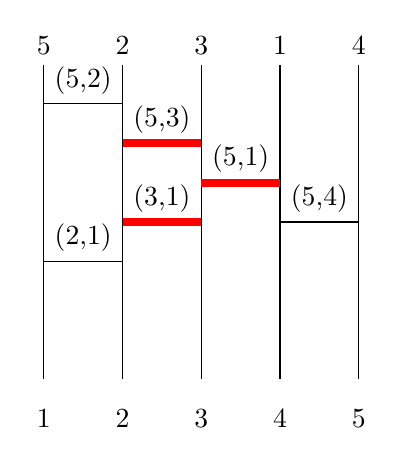
\begin{tikzpicture}
				\draw(0, 0) to (0, 4) node[above]{5};
				\node at (0, -0.5){1};

				\draw(1, 0) to (1, 4) node[above]{2};
				\node at (1, -0.5){2};


				\draw(2, 0) to (2, 4) node[above]{3};
				\node at (2, -0.5){3};

				\draw(3, 0) to (3, 4) node[above]{1};
				\node at (3, -0.5){4};


				\draw(4, 0) to (4, 4) node[above]{4};
				\node at (4, -0.5){5};

				%%drawing the bars

				%%5's route
				\draw(0, 3.5)to (1, 3.5);
					\draw node at (0.5, 3.8) {(5,2)};
				\draw[line width=1mm, red](1, 3) to (2, 3);
					\draw node at (1.5, 3.3) {(5,3)};
				\draw[line width=1mm, red](2, 2.5) to (3, 2.5);
					\draw node at (2.5, 2.8) {(5,1)};
				\draw(3, 2) to (4, 2);
					\draw node at (3.5, 2.3) {(5,4)};

				%%4's route, no bars

				%%3s route
				\draw[line width=1mm, red](1, 2) to (2, 2);
					\draw node at (1.5, 2.3) {(3,1)};
				%%2s route
				\draw(0, 1.5) to (1, 1.5);
					\draw node at (0.5, 1.8){(2,1)};

			\end{tikzpicture}
		\end{center}
	\end{minipage}
	\begin{minipage}{0.4\textwidth}
		\begin{flushright}

			%%drawing the lines
			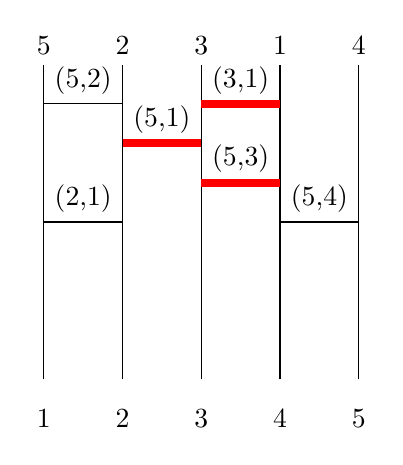
\begin{tikzpicture}
				\draw(0, 0) to (0, 4) node[above]{5};
				\node at (0, -0.5){1};

				\draw(1, 0) to (1, 4) node[above]{2};
				\node at (1, -0.5){2};


				\draw(2, 0) to (2, 4) node[above]{3};
				\node at (2, -0.5){3};

				\draw(3, 0) to (3, 4) node[above]{1};
				\node at (3, -0.5){4};


				\draw(4, 0) to (4, 4) node[above]{4};
				\node at (4, -0.5){5};

				%%Drawing the bars
				\draw(0, 3.5)to (1, 3.5);
					\draw node at (0.5, 3.8){(5,2)};
				\draw[line width=1mm, red](2, 3.5) to (3, 3.5);
					\draw node at (2.5, 3.8) {(3,1)};
				\draw[line width=1mm, red](2, 2.5) to (3, 2.5);
					\draw node at (2.5, 2.8) {(5,3)};
				\draw(3, 2) to (4, 2);
					\draw node at (3.5, 2.3){(5,4)};
				%%4's route, no bars

				%%3s route
				\draw[line width=1mm, red](1, 3) to (2, 3);
					\draw node at (1.5, 3.3) {(5,1)};
				%%2s route
				\draw(0, 2) to (1, 2);
					\draw node at(0.5, 2.3){(2,1)};
			\end{tikzpicture}
		\end{flushright}
	\end{minipage}
	\caption{Example of a local swap operation. When a right swap operation is performed
	on the left ladder, the result is the right ladder. When a left swap operation is performed
	on the right ladder, the result is the left ladder.}
	\label{fig:rightSwap}
\end{figure}

\par

%%%%%%%%%%%%%%%%%%%%%%%%%%%%%%%FIND ALL CHILDREN ALGORITHM%%%%%%%%%%%%%%%%%%%%%%%%%%%%%



%%%%%%%%%%%%%%%%%%END ALGORITHM%%%%%%%%%%%%%%%%%%%%%%%%%%



{\sc {\sc FindAllChildren}} was used in this thesis to generate the sample data that aided in finding solutions for 
the Gray Code Problem in Chapter 3 and the Minimum Height Problem in Chapter 4.  
Therefore, this algorithm is paramount for the findings of this thesis. 
To see the tree structure generated by {\sc FindAllChildren} for $OptL\{(4,3,2,1)\}$ 
please refer to Figure~\ref{Fig:TreeFAC}. 
\begin{figure}[h]
	\centering 
	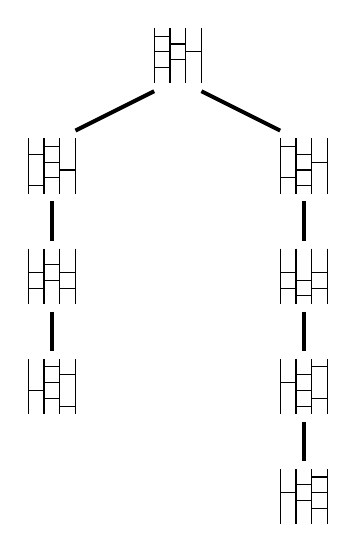
\begin{tikzpicture}
		%%L1
		\draw(5, 10) to (5, 9.3);
			\draw(5, 9.9) to (5.2, 9.9);
			\draw(5.2, 9.8) to (5.4, 9.8);
			\draw(5.4, 9.7) to (5.6, 9.7);
		\draw(5.2, 10) to (5.2, 9.3);
			\draw(5, 9.7) to (5.2, 9.7);
			\draw(5.2, 9.6) to (5.4, 9.6);
		\draw(5.4, 10) to (5.4, 9.3);
			\draw(5, 9.5) to (5.2, 9.5);
		\draw(5.6, 10) to (5.6, 9.3);
		%L2
		\draw[line width = .5mm](5, 9.2) to (4, 8.7);
		\draw[line width = .5mm](5.6, 9.2) to (6.6, 8.7);
			%%L2
			\draw(3.4, 8.6) to (3.4, 7.9);
				\draw(3.4, 8.4) to (3.6, 8.4);
				\draw(3.4, 8) to (3.6, 8);
			\draw(3.6, 8.6) to (3.6, 7.9);
				\draw(3.6, 8.5) to (3.8, 8.5);
				\draw(3.6, 8.3) to (3.8, 8.3);
				\draw(3.6, 8.1) to (3.8, 8.1);
			\draw(3.8, 8.6) to (3.8, 7.9);
				\draw(3.8, 8.2) to (4, 8.2);
			\draw(4.0, 8.6) to (4.0, 7.9);

				%%level
				\draw[line width = .5mm](3.7, 7.8) to (3.7, 7.3);
			\draw(3.4, 7.2) to (3.4, 6.5);
				\draw(3.4, 6.9) to (3.6, 6.9);
				\draw(3.4, 6.7) to (3.6, 6.7);
			\draw(3.6, 7.2) to (3.6, 6.5);
				\draw(3.6, 7) to (3.8, 7);
				\draw(3.6, 6.8) to (3.8, 6.8);
			\draw(3.8, 7.2) to (3.8, 6.5);
				\draw(3.8, 6.9) to (4, 6.9);
				\draw(3.8, 6.7) to (4, 6.7);
			\draw(4.0, 7.2) to (4.0, 6.5);

		%%L3
			\draw(6.6, 8.6) to (6.6, 7.9);
				\draw(6.6, 8.5) to (6.8, 8.5);
				\draw(6.8, 8.4) to (7, 8.4);
				\draw(7, 8.3) to (7.2, 8.3);
			\draw(6.8, 8.6) to (6.8, 7.9);
				\draw(6.8, 8.2) to (7, 8.2);
				\draw(6.8, 8) to (7, 8);
			\draw(7, 8.6) to (7, 7.9);
				\draw(6.6, 8.1) to (6.8, 8.1);
			\draw(7.2, 8.6) to (7.2, 7.9);
			
			
			\draw[line width = .5mm](6.9, 7.8) to (6.9, 7.3);

			\draw(6.6, 7.2) to (6.6, 6.5);
				\draw(6.6, 6.9) to (6.8, 6.9);
				\draw(6.6, 6.7) to (6.8, 6.7);
			\draw(6.8, 7.2) to (6.8, 6.5);
				\draw(6.8, 6.8) to (7, 6.8);
				\draw(6.8, 6.6) to (7, 6.6);
			\draw(7.0, 7.2) to (7.0, 6.5);
				\draw(7, 6.9) to (7.2, 6.9);
				\draw(7, 6.7) to (7.2, 6.7);
			\draw(7.2, 7.2) to (7.2, 6.5);

			\draw[line width = .5mm](3.7, 6.4) to (3.7, 5.9);

			\draw(3.4, 5.8) to (3.4, 5.1);
				\draw(3.4, 5.4) to (3.6, 5.4);
			\draw(3.6, 5.8) to (3.6, 5.1);
				\draw(3.6, 5.7) to (3.8, 5.7);

				\draw(3.6, 5.5) to (3.8, 5.5);
				\draw(3.6, 5.3) to (3.8, 5.3);
			\draw(3.8, 5.8) to (3.8, 5.1);
				\draw(3.8, 5.6) to (4, 5.6);
				\draw(3.8, 5.2) to (4, 5.2);
			\draw(4.0, 5.8) to (4.0, 5.1);

			\draw[line width = .5mm](6.9, 6.4) to (6.9, 5.9);

			
			\draw(6.6, 5.8) to (6.6, 5.1);
				\draw(6.6, 5.5) to (6.8, 5.5);
			\draw(6.8, 5.8) to (6.8, 5.1);
				\draw(6.8, 5.6) to (7, 5.6);

				\draw(6.8, 5.4) to (7, 5.4);
				\draw(6.8, 5.2) to (7, 5.2);
			\draw(7.0, 5.8) to (7.0, 5.1);
				\draw(7.0, 5.7) to (7.2, 5.7);
				\draw(7.0, 5.3) to (7.2, 5.3);
			\draw(7.2, 5.8) to (7.2, 5.1);

			\draw[line width = .5mm](6.9, 5) to (6.9, 4.5);

			\draw(6.6, 4.4) to (6.6, 3.7);
				\draw(6.6, 4.1) to (6.8, 4.1);
			\draw(6.8, 4.4) to (6.8, 3.7);
				\draw(6.8, 4.2) to (7, 4.2);

				\draw(6.8, 4) to (7, 4);
			\draw(7.0, 4.4) to (7.0, 3.7);
				\draw(7.0, 4.3) to (7.2, 4.3);
				\draw(7.0, 4.1) to (7.2, 4.1);
				\draw(7.0, 3.9) to (7.2, 3.9);
			\draw(7.2, 4.4) to (7.2, 3.7);



	\end{tikzpicture}
	\caption{The tree structure of $OptL\{(4,3,2,1)\}$ generated by {\sc FindAllChildren}}
	\label{Fig:TreeFAC}
\end{figure}
\pagebreak
{\sc FindAllChildren} is based on several key concepts. One of which is the local swap operation 
which has already been discussed. The next fundamental concept is the \emph{route} of an element, 
which is the sequence of bars the element travels along in order to reach its final position in the 
sorted permutation. The bars are read from top to bottom. For every bar, two elements cross 
the bar, therefore the bar is associated with the route of the greater of the two elements~\cite{A1}. 
In Figure~\ref{Fig:Route} the route of element $4$ is the sequence of bars 
$(4,1),(4,2),(5,4)$. To see the route of an element please refer to Figure~\ref{Fig:Route}. When a 
right swap operation occurs, the bar of the route associated with a lesser element is 
swapped above two bars of a route associated with a greater element. For example, in Figure~\ref{fig:rightSwap} in the right ladder, 
the bar $(3,1)$ which is associated with the route of element $3$ is right swapped above the two bars $(5,1)$ and $(5,3)$ 
both of which are associated with the route of $5$.\par 
\begin{figure}[h]
	\centering
	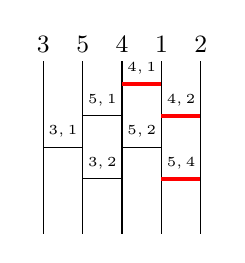
\begin{tikzpicture}
		\draw(0, 0) to (0, 2.2);
			\node at(.25, 1.3){\tiny{$3,1$}};
			\draw(0, 1.1) to (.5, 1.1);
		\draw(.5, 0) to (.5, 2.2);
			\node at(.75, 1.7){\tiny{$5,1$}};
			\draw(.5, 1.5) to (1, 1.5);
			\node at(.75, .9){\tiny{$3,2$}};
			\draw(.5, .7) to (1, .7);
		\draw(1, 0) to (1, 2.2);
			\node at(1.25, 2.1){\tiny{$4,1$}};
			\draw[line width=.5mm, red ](1, 1.9) to (1.5, 1.9);
			\node at(1.25, 1.3){\tiny{$5,2$}};
			\draw(1, 1.1) to(1.5, 1.1);
		\draw(1.5, 0) to (1.5, 2.2);
			\node at(1.75, 1.7){\tiny{$4,2$}};
			\draw[line width=.5mm, red ](1.5, 1.5) to (2, 1.5);
			\node at(1.75, .9){\tiny{$5,4$}};
			\draw[line width=.5mm, red ](1.5, .7) to (2, .7);
		\draw(2, 0) to (2, 2.2);


		\node at(0.0, 2.4){\small{$3$}};
		\node at(0.5, 2.4){\small{$5$}};
		\node at(1.0, 2.4){\small{$4$}};
		\node at(1.5, 2.4){\small{$1$}};
		\node at(2.0, 2.4){\small{$2$}};
	\end{tikzpicture}
	\caption{The route of element 4=(4,1),(4,2),(5,4).}
	\label{Fig:Route}
\end{figure}



The \emph{clean level} is defined as one more than the largest 
element associated with any bar that has undergone a right swap operation. 
For example, if the largest element associated with a bar that has undergone a 
right swap operation is element $4$, then the clean level is $5=4+1$.
 Please refer to Figure~\ref{Fig:CleanLevel} for an example of the clean level.
 If no bars have been right swapped, then the clean level is $1$.
If the largest element to have undergone a right swap operation is the maximal element in $\pi$, 
then the clean level is $max+1$.\pagebreak

\begin{figure}[t]
	\centering 
	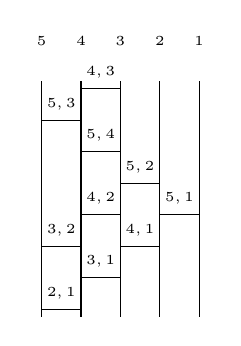
\begin{tikzpicture}
		\draw(0, 0) to (0, 3);
			\node at(.25, 2.7){\tiny{$5,3$}};
			\node at(.25, 1.1){\tiny{$3,2$}};
			\node at(.25, .3){\tiny{$2,1$}};
			\draw(0, 2.5) to (.5, 2.5);			
			\draw(0, .9) to (.5, .9);
			\draw(0, .1) to (.5, .1);

		\draw(.5, 0) to (.5, 3);
			\node at(.75, 3.1){\tiny{$4,3$}};
			\node at(.75, 2.3){\tiny{$5,4$}};
			\node at(.75, 1.5){\tiny{$4,2$}};
			\node at(.75, .7){\tiny{$3,1$}};

			\draw(.5, 2.9) to (1, 2.9);
			\draw(.5, 2.1) to (1, 2.1);
			\draw(.5, 1.3) to (1, 1.3);
			\draw(.5, .5) to (1, .5);
		\draw(1, 0) to (1, 3);
			\node at(1.25, 1.9){\tiny{$5,2$}};
			\node at(1.25, 1.1){\tiny{$4,1$}};

			\draw(1, 1.7) to (1.5, 1.7);
			\draw(1, .9) to (1.5, .9);
		\draw(1.5, 0) to (1.5, 3);
			\node at(1.75, 1.5){\tiny{$5,1$}};
			\draw(1.5, 1.3) to (2, 1.3);
		\draw(2, 0) to (2, 3);

		%%%%%%%%%%%%%%%%%%%%%%%%%%%%
		\node at(0, 3.5){\tiny{$5$}};
		\node at(.5, 3.5){\tiny{$4$}};
		\node at(1, 3.5){\tiny{$3$}};
		\node at(1.5, 3.5){\tiny{$2$}};
		\node at(2, 3.5){\tiny{$1$}};
\end{tikzpicture}
	\caption{A ladder with a clean level of $6$. The largest element whose associated bars have undergone a right swap operation is $5$}
	\label{Fig:CleanLevel}
\end{figure}


Each $OptL\{\pi\}$ has a unique ladder with a clean level of one. This ladder 
is known as the \emph{root ladder}. To see the root ladder 
of $OptL\{(4,5,6,3,1,2)\}$ please refer to figure Figure~\ref{fig:root}. To see a proof 
for the uniqueness of the root ladder please refer to Theorem~\ref{Theorem:One}.

%%%%%%%%%%%%%ROOT LADDER FIGURE%%%%%%%%%%%%%%%%%%%%%%%
\begin{figure}[h]


	\begin{center}
		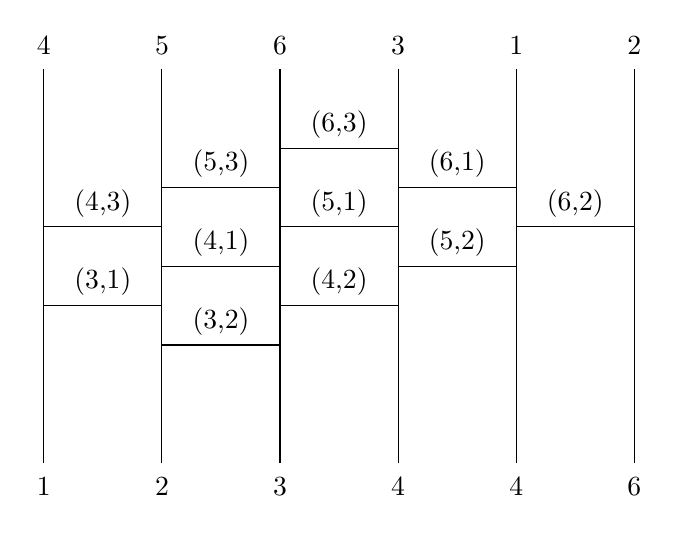
\begin{tikzpicture}
			%%draw the lines
			\draw(0, 0) to (0, 5);
				\node at (0, 5.3){4};
				\node at (0, -0.3){1};

			\draw(1.5, 0) to (1.5, 5);
				\node at (1.5, 5.3){5};
				\node at (1.5, -0.3){2};
			
			\draw(3, 0) to (3, 5);
				\node at (3, 5.3){6};
				\node at (3, -0.3){3};
			\draw(4.5, 0) to (4.5, 5);
				\node at (4.5, 5.3){3};
				\node at (4.5, -0.3){4};
			\draw(6, 0) to (6, 5);
				\node at (6, 5.3){1};
				\node at (6, -0.3){4};
			\draw(7.5, 0) to (7.5, 5);
				\node at (7.5, 5.3){2};
				\node at (7.5, -0.3){6};

			%%draw the bars
			
			%%6's route
			\draw(3, 4) to (4.5, 4);
				\node at (3.75, 4.3){(6,3)};
			\draw(4.5, 3.5) to (6, 3.5);
				\node at (5.25, 3.8){(6,1)};
			\draw(6, 3) to (7.5, 3);
				\node at (6.75, 3.3){(6,2)};
			%%5's route
			\draw(1.5, 3.5) to (3, 3.5);
				\node at (2.25, 3.8){(5,3)};
			\draw(3, 3) to (4.5, 3);
				\node at (3.75, 3.3){(5,1)};
			\draw(4.5, 2.5) to (6, 2.5);
				\node at (5.25, 2.8){(5,2)};
			%draw 4's route
			\draw(0, 3) to (1.5, 3);
				\node at (0.75, 3.3){(4,3)};
			\draw(1.5, 2.5) to (3, 2.5);
				\node at (2.25, 2.8){(4,1)};
			\draw(3, 2) to (4.5, 2);
				\node at (3.75,2.3){(4,2)};

			%%draw 3's route
			\draw(0, 2) to (1.5, 2);
				\node at (0.75, 2.3){(3,1)};
			\draw(1.5, 1.5) to (3, 1.5);
				\node at (2.25, 1.8){(3,2)};
		\end{tikzpicture}

	\end{center}





	\caption{The root ladder for $OptL\{(4,5,6,3,1,2)\}$. Notice how 
	no bar associated with a lesser element is above bars associated with a greater element.
	Therefore, the clean level of this ladder is $1$, thus making it the root ladder.} 
	\label{fig:root}

\end{figure}

\begin{theorem}
	 The root ladder is unique to $OptL\{\pi\}$. 
	 \label{Theorem:One}
 \end{theorem} 
 \begin{proof}
	Since the parent to child relation of the tree structure generated by {\sc FindAllChildren} is based on a right swap operation 
	and the child to parent relation of the tree structure generated by {\sc FindAllChildren} is based on a left swap operation, then 
	there exists a ladder in the tree structure such that no bars have been right swapped. 
	If this were not the case, then we affirm an infinite regress. 
	Thus, there exists a ladder in the tree structure that is not derived from a right swap operation. This ladder 
	is the root ladder seeing as once a right swap operation has occurred, the clean level of the ladder 
	ceases to equal one. But we have already stated that the clean level of the root ladder is one. Therefore, 
	this ladder must be the root ladder. To prove that 
	the root ladder is unique, consider that we are dealing with a tree structure. Trees have a single 
	root. The root in the tree structure for $OptL\{\pi\}$ is the ladder that has not undergone any right swap operations.
	Thus, the root ladder is the unique root of the tree structure generated by {\sc FindAllChildren}.
   
 \end{proof}
 \begin{corollary}
	 If $|OptL\{\pi\}|=1$ then the ladder in $OptL\{\pi\}$ must be the root ladder.
 \end{corollary}
 \begin{proof}
	 If there is only one ladder in the set, then that means no bars have been swapped in said ladder. 
	 Thus, it must be the root ladder.
 \end{proof}

%%Root ladder subsection
The authors provide a good description of the foundational concepts required to 
generate $OptL\{\pi\}$ using {\sc FindAllChildren}. However, the authors do not provide 
an algorithm for performing a local swap operation nor do they provide an algorithm for creating the root ladder.
In order to effectively implement {\sc FindAllChildren}, algorithms for creating the root ladder and performing 
local swap operations are necessary.
Seeing as the root ladder cannot be created by performing a right swap operation, a separate 
algorithm is required for creating the root ladder. This thesis provides 
novel algorithms for creating the root ladder and for performing a local swap operation.
Please refer to Algorithm~\ref{Alg:RootLadder} to see the algorithm for creating 
the root ladder. The initial conditions of Algorithm~\ref{Alg:RootLadder} are the 
following. Let $ladder$ be initialized to an empty ladder. Let $n$ be initialized 
to {\sc Max($\pi$)}. Let $row$ be initialized to one. $\pi$ is an arbitrary permutation 
of order $n$.
\begin{algorithm}[!htp]
	\begin{algorithmic}[1]
		\Function {CreateRoot}{$ladder$, $\pi$, $n$, $row$}
			\If{$n=1$}
				\State return
			\EndIf
			\State $x \gets$ index of {\sc Max($\pi$)}
			\For{$i \gets x+1$ \textbf{to} $n$}
				\If{$p_{x}>p_{i}$ \textbf{and} $x<i$}
					\State $column \gets i$
					\If{this is the first bar to be added}
						\While{bar cannot be added}
							\State $row \gets row+1$
						\EndWhile
						\State $ladder[row][column] \gets 1$
					\Else 
						\State $row \gets row+1$
						\State $ladder[row][column] \gets 1$
					\EndIf
				\EndIf
			\EndFor
			\State $\pi \gets \pi - largestElement$
			\State {\sc CreateRoot($ladder$, $\pi$, $n-1$, $row \gets 1$)}
		\EndFunction

	\end{algorithmic}
	\caption{The algorithm for creating the root ladder of $OptL\{\pi\}$}
	\label{Alg:RootLadder}
\end{algorithm}\pagebreak



Let $ladder$ be a two dimensional array, let $\pi$ be the current state of the permutation, let $row$ be the current row in the ladder. 
First, the index of the largest element in $\pi$ is assigned to $x$. 
Once found, the algorithm loops from $x+1$ to $n$. If $p_{x}>p_{i}$ then a bar is to be added to 
$ladder$ at $row,column=i$. There are two cases for calculating the $row$. 
\case{\emph{First bar is being added}}{This is the first bar to be added to the route of the largest element. 
$row$ is incremented until a bar can be added to $ladder$ at $row$ 
and $column$. A bar can be added if neither of its endpoints are touching the endpoints of any other bar.}
\case{\emph{Second or greater bar is being added}}{If this is second or greater bar to be added to the route of the 
largest element in $\pi$ then $row \gets row+1$.}
Once all the bars for the route of the largest element have been added, the largest element from $\pi$ is removed; 
$\pi \gets \pi -$ {\sc max($\pi$)}. $n \gets n-1$ and $row \gets 1$. The algorithm then makes a recursive call.

\begin{lemma}
	The time complexity for CreateRoot is $O(n^{3})$
\end{lemma}
\begin{proof}
	The outer for-loop of the function runs from some arbitrary index to $n$ on each function call. The inner for loop runs at most 
	$2(n-1)-1$ times which is reduced to $n$. Thus, we get $O(n^{2})$. The following 
	recursion holds, $CreateRoot(n-k) = CreateRoot(n-k+1) + O((n-k)^{2})=(CreateRoot(n-k+2) + O((n-k+1)^{2})) + O((n-k)^{2})\dots $. Which is 
	reduced to $O(n(n+1)(2n+1)/6) = O(n^3)$.
\end{proof}
\pagebreak
The following algorithms are used to perform a local swap operation: Algorithm~\ref{Alg:RightSwap}, Algorithm~\ref{Alg:LeftSwap} and Algorithm~\ref{Alg:ShiftSubLadder}.
Let $ladder$ be initialized to an empty ladder. Let $bar$ be the bar to be right or left swapped in the $ladder$.
In Algorithm~\ref{Alg:ShiftSubLadder} \textit{offset} is initialized to $2$ when right swapping and initialized to 
$-2$ when left swapping. In Algorithm~\ref{Alg:ShiftSubLadder} \textit{index} is initialized to $1$ when 
right swapping and $-1$ when left swapping.
Let the \emph{right child} of some arbitrary bar $w$, $rc(w)$ for short, be the bar one row below, and one column to the 
right of $w$. Let the \emph{left child} of some arbitrary bar $w$, $lc(w)$ for short, be the bar one 
row below, and one column to the left of $w$. 
Let the \emph{right sibling} of $w$, $rs(w)$ for short,  be defined as the bar on the same row as some arbitrary bar $w$ and
two columns to the right of bar $w$. 
Let the \emph{upper neighbor} of $w$, $un(w)$ for short, be the bar that is two rows above the row of $w$ and is 
in the same column as $w$. Let the \emph{right neighbor} of $w$, $rn(w)$ for short, be the bar that is one row 
above $w$ and one column to the right of $w$. Let the lower neighbor of $w$, $ln(w)$ for short be 
the bar that is two rows below $w$ and in the same column as $w$. Let the left neighbor of 
$w$, $lfn(n)$ for short, be the bar one row below and one column to the left of $w$.
Let the \emph{sub-ladder} be a subset of bars such that each bar in the sub-ladder is a left or right child 
of some other bar in the sub-ladder except the root of the sub-ladder. For an example of a sub-ladder please refer to 
Figure~\ref{Figure:Sub-ladder}.
\begin{figure}[h]
	\centering
	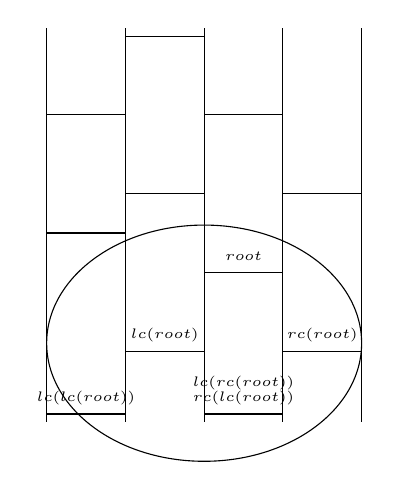
\begin{tikzpicture}
		\draw(0, 0) to (0, 5);
			\draw(0, 3.9) to (1, 3.9);
			\draw(0, 2.4) to (1, 2.4);
			\node at(.5, .3){\tiny{$lc(lc(root))$}};
			\draw(0, 0.1) to (1, 0.1);
		\draw(1, 0) to (1, 5);
			\draw(1, 4.9) to (2, 4.9);
			\draw(1, 2.9) to (2, 2.9);
			\node at(1.5, 1.1){\tiny{$lc(root)$}};
			\draw(1, 0.9) to (2, 0.9);
		\draw(2, 0) to (2, 5);
			\draw(2, 3.9) to (3, 3.9);
			\node at(2.5, 2.1){\tiny{$root$}};
			\draw(2, 1.9) to (3, 1.9);
			\node at(2.5, .3){\tiny{$rc(lc(root))$}};
			\node at(2.5, .5){\tiny{$lc(rc(root))$}};
			\draw(2, 0.1) to (3, 0.1);
		\draw(3, 0) to (3, 5);
			\draw(3, 2.9) to (4, 2.9);
			\node at(3.5,1.1){\tiny{$rc(root)$}};
			\draw(3, 0.9) to (4, 0.9);
		\draw(4, 0) to (4, 5);

		\draw (2, 1) ellipse (2cm and 1.5cm);
	\end{tikzpicture}

	\caption{The bars that are fully or partially in the circle make up the sub-ladder.}
	\label{Figure:Sub-ladder}
	
\end{figure}

%%%%%%% ALGORITHM RIGHT SWAP %%%%%%%%%%%%%%%%%%%
\begin{algorithm}[!htp]
	\begin{algorithmic}[1]
		\Function{RightSwap}{$ladder$, $bar$}
			\State $row \gets bar's$ row in $ladder$
			\State $col \gets bar's$ column in $ladder$
			\State $upperNeighbor \gets un(bar)$
			\State $rightNeighbor \gets rn(bar)$
			\If{$col<=n-3$}
				\State $subLadderRoot \gets$ $rs(bar)$
				\State {\sc ShiftSubLadder($ladder$, $subLadderRoot$, 2)}
			\EndIf
			\State {\sc Swap($upperNeighbor$, $ladder[row+1][col+1]$)}
			\State {\sc Swap($bar$, $rightNeighbor$)}
		\EndFunction
	\end{algorithmic}
	\caption{Perform a right swap operation on a bar}
	\label{Alg:RightSwap}
\end{algorithm}


%%%%%%%%%% ALGORITHM LEFT SWAP %%%%%%%%%%%%%%%%%%%%%%%%
\begin{algorithm}[!htp]
	\begin{algorithmic}[1]
		\Function{LeftSwap}{$ladder$, $bar$}
			\State $row \gets bar's$ row in ladder 
			\State $col \gets bar's$ column in ladder
			\State $leftNeighbor \gets lfn(bar)$
			\State {\sc Swap($bar$, $leftNeighbor$)}
			\State $lowerNeighbor \gets ln(bar)$
			\If{$col<n-1$}
				\State $subLadderRoot \gets$ $rc(lowerNeighbor)$
				\State {\sc Swap($lowerNeighbor$, $ladder[row-1][col-1]$)}
				\State {\sc ShiftSubLadder($ladder$, $subLadderRoot$, $-2$)}
			\Else 
				\State {\sc Swap($lowerNeighbor$, $ladder[row-1][col-1]$)}
			\EndIf
		\EndFunction
	\end{algorithmic}
	\caption{Perform a left swap operation on a bar}
	\label{Alg:LeftSwap}
\end{algorithm}


%%%%%%%%%%%% ALGORITHM ShiftSubLadderDOWN %%%%%%%%%%%%%%%%%%%%%%
\begin{algorithm}[!htp]
	\begin{algorithmic}[1]
		\Function{ShiftSubLadder}{$ladder$, $bar$, \textit{offset}}
			\State $row \gets bar's$ row in ladder
			\State $col \gets bar's$ column in ladder
			\State $rightChild \gets rc(bar)$
			\State $leftChild \gets lc(bar)$
			\If{$rightChild=0$ \textbf{and} $leftChild=0$}
				\State {\sc Swap($ladder[row+$\textit{offset}$][col]$, $ladder[row][col]$)}
				\State \textbf{return}
			\Else 
				\If{\textit{offset}$==-2$ indicating a left swap}
					\State {\sc Swap($ladder[row+$\textit{offset}$][col]$, $ladder[row][col]$)}
					\If{$rightChild \neq 0$}
						\State {\sc ShiftSubLadder($ladder$, $rightChild$, \textit{offset})}
					\EndIf 
					\If{$leftChild \neq 0$}
						\State {\sc ShiftSubLadder($ladder$, $leftChild$, \textit{offset})}
					\EndIf
				\EndIf
				\If{\textit{offset}$==2$ indicating a right swap}
					\If{$rightChild \neq 0$}
						\State {\sc ShiftSubLadder($ladder$, $rightChild$, \textit{offset})}
					\EndIf 
					\If{$leftChild \neq 0$}
						\State {\sc ShiftSubLadder($ladder$, $leftChild$, \textit{offset})}
					\EndIf 
					\State {\sc Swap($ladder[row+$\textit{offset}$][col]$, $ladder[row][col]$)}
				\EndIf
			\EndIf
		\EndFunction
	\end{algorithmic}
	\caption{Shifts the sub-ladder up or down the ladder data structure depending on if a right or left swap operation is being performed}
	\label{Alg:ShiftSubLadder}
\end{algorithm}\pagebreak


The way that the aforementioned three algorithms work in order 
to complete a local swap operation is as follows. 
When performing a right swap operation, {\sc RightSwap}
takes the current bar, $x$, and gets its upper neighbor $z$ and its right neighbor $y$; $x$, $z$ and $y$ meet the 
criteria for performing a right swap operation. Then, {\sc RightSwap} calls {\sc ShiftSubLadder}
with the \emph{offset} value of $2$ and the \emph{index} value of one. 
Algorithm {\sc ShiftSubLadder} ensures that the bottom right sub-ladder, beginning at the right sibling of $x$/$rs(x)$, 
is shifted down the ladder such that when the right 
swap operation is performed, the root of the sub-ladder is the right child of $z$. 
When performing a right swap, {\sc ShiftSubLadder} moves each bar in the sub-ladder two rows 
down the ladder. Since each bar in the sub-ladder is a left or right child of some other bar in the sub-ladder, 
with the exception of the root ladder, the index is set to $1$ indicating the offset.
When a right swap operation is about to occur, bar $z$ will be moved from its current row and column to its current row + $3$ 
and its current column $+1$. Once the right swap operation is performed, 
$rs(x)$ becomes $rc(z)$. $y$ and $x$ are swapped. Then the function is complete.\par 

%%%%%%%%%FIX ME%%%%%%%%%%%%%%%%%%%%%%%%
The left swap operation reverses the resulting ladder from the right swap operation; {\sc LeftSwap}
is the inverse of {\sc RightSwap}. The \textit{offset} value for {\sc ShiftSubLadder} when 
performing a left swap is set to $-2$ to indicate the bars need to be moved up the ladder. 
When bars are moved in {\sc LeftSwap}, the parent bar is shifted upward before its children.
This is unlike the {\sc RightSwap} in which the children bars are shifted downward 
before their parent. This is done to ensure that for any two bars in the sub-ladder, 
$x,y$, $x$ will not be swapped with $y$, thus putting $y$ in the wrong position. 
This is why the $lowerNeighbor$ of $x$ in {\sc LeftSwap} is swapped before 
{\sc ShiftSubLadder} is called. Whereas in {\sc RightSwap} the $upperNeighbor$ 
of $x$ is swapped after {\sc ShiftSubLadder} is called.
To see an example of all three algorithms performing a local swap operation please refer to Figure \ref{Fig:SwapAndShift}.\pagebreak
\begin{figure}[!htp]
	\begin{minipage}{.4\textwidth}
		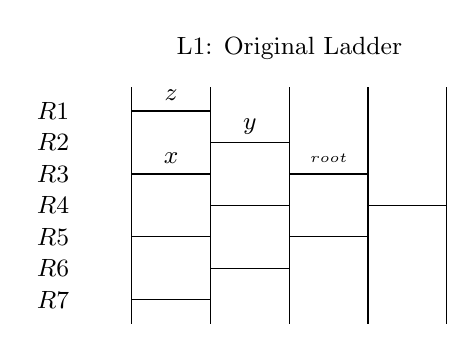
\begin{tikzpicture}
			\node at(2, 3.5){\small{L1: Original Ladder}};
			\draw(0, 0) to (0, 3);
					\node at(.5, 2.9){\small{$z$}};
				\draw(0, 2.7) to (1,2.7);
					\node at(.5, 2.1){\small{$x$}};

				\draw(0,1.9) to (1,1.9);
				\draw(0,1.1) to (1,1.1);
				\draw(0,0.3) to (1,0.3);
			\draw(1, 0) to (1, 3);
				\node at(1.5,2.5){\small{$y$}};
				\draw(1,2.3) to (2,2.3);
				\draw(1,1.5) to (2,1.5);
				\draw(1,0.7) to (2,0.7);
			\draw(2, 0) to (2, 3);
				\node at(2.5, 2.1){\tiny{$root$}};
				\draw(2,1.9) to (3,1.9);
				\draw(2,1.1) to (3,1.1);
			\draw(3, 0) to (3, 3);
				\draw(3,1.5) to (4,1.5);
			\draw(4, 0) to (4, 3);

			\node at(-1, 2.7){\small{$R1$}};
			\node at(-1, 2.3){\small{$R2$}};
			\node at(-1, 1.9){\small{$R3$}};
			\node at(-1, 1.5){\small{$R4$}};
			\node at(-1, 1.1){\small{$R5$}};
			\node at(-1, .7){\small{$R6$}};
			\node at(-1, .3){\small{$R7$}};

			
		\end{tikzpicture}
	\end{minipage}
	\begin{minipage}{.4\textwidth}
		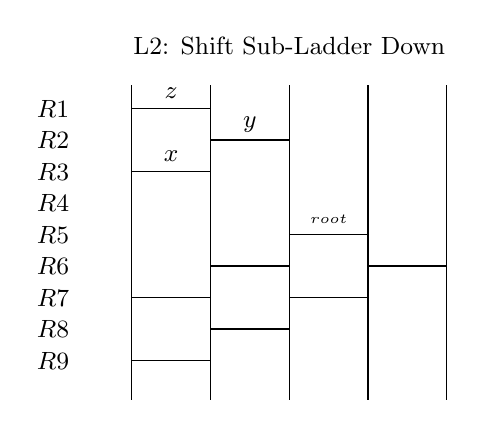
\begin{tikzpicture}
			\node at(2, 3.5){\small{L2: Shift Sub-Ladder Down}};

			\draw(0, -1) to (0, 3);
					\node at(.5, 2.9){\small{$z$}};
				\draw(0, 2.7) to (1,2.7);
					\node at(.5, 2.1){\small{$x$}};

				\draw(0,1.9) to (1,1.9);
				\draw(0,.3) to (1,.3);
				\draw(0,-0.5) to (1,-0.5);
			\draw(1, -1) to (1, 3);
				\node at(1.5,2.5){\small{$y$}};
				\draw(1,2.3) to (2,2.3);
				\draw(1,0.7) to (2,0.7);
				\draw(1,-0.1) to (2,-0.1);
			\draw(2, -1) to (2, 3);
				\node at(2.5, 1.3){\tiny{$root$}};
				\draw(2,1.1) to (3,1.1);
				\draw(2,.3) to (3,.3);
			\draw(3, -1) to (3, 3);
				\draw(3,.7) to (4,.7);
			\draw(4, -1) to (4, 3);

			\node at(-1, 2.7){\small{$R1$}};
			\node at(-1, 2.3){\small{$R2$}};
			\node at(-1, 1.9){\small{$R3$}};
			\node at(-1, 1.5){\small{$R4$}};
			\node at(-1, 1.1){\small{$R5$}};
			\node at(-1, .7){\small{$R6$}};
			\node at(-1, .3){\small{$R7$}};
			\node at(-1, -.1){\small{$R8$}};
			\node at(-1, -.5){\small{$R9$}};


			
		\end{tikzpicture}
	\end{minipage}
	\begin{minipage}{.4\textwidth}
		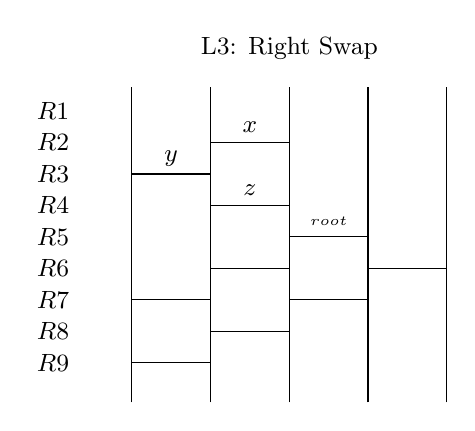
\begin{tikzpicture}
			\node at(2, 3.5){\small{L3: Right Swap}};

			\draw(0, -1) to (0, 3);
					\node at(1.5, 1.7){\small{$z$}};
				
					\node at(.5, 2.1){\small{$y$}};

				\draw(0,1.9) to (1,1.9);
				\draw(0,.3) to (1,.3);
				\draw(0,-0.5) to (1,-0.5);
			\draw(1, -1) to (1, 3);
				\node at(1.5,2.5){\small{$x$}};
				\draw(1,2.3) to (2,2.3);
				\draw(1, 1.5) to (2,1.5);
				\draw(1,0.7) to (2,0.7);
				\draw(1,-0.1) to (2,-0.1);
			\draw(2, -1) to (2, 3);
				\node at(2.5, 1.3){\tiny{$root$}};
				\draw(2,1.1) to (3,1.1);
				\draw(2,.3) to (3,.3);
			\draw(3, -1) to (3, 3);
				\draw(3,.7) to (4,.7);
			\draw(4, -1) to (4, 3);

			\node at(-1, 2.7){\small{$R1$}};
			\node at(-1, 2.3){\small{$R2$}};
			\node at(-1, 1.9){\small{$R3$}};
			\node at(-1, 1.5){\small{$R4$}};
			\node at(-1, 1.1){\small{$R5$}};
			\node at(-1, .7){\small{$R6$}};
			\node at(-1, .3){\small{$R7$}};
			\node at(-1, -.1){\small{$R8$}};
			\node at(-1, -.5){\small{$R9$}};


			
		\end{tikzpicture}
	\end{minipage}
	\hfill
	\begin{minipage}{.4\textwidth}
		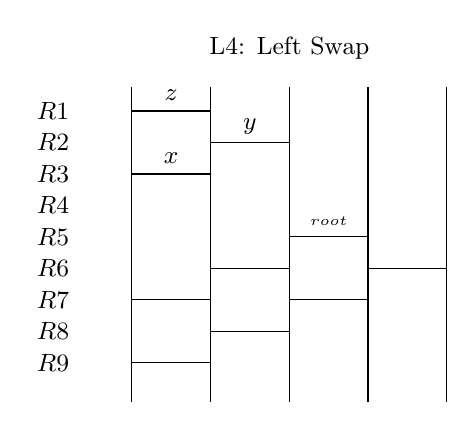
\begin{tikzpicture}
			\node at(2, 3.5){\small{L4: Left Swap}};

			\draw(0, -1) to (0, 3);
					\node at(0.5, 2.9){\small{$z$}};
				
					\node at(.5, 2.1){\small{$x$}};

				\draw(0,1.9) to (1,1.9);
				\draw(0,.3) to (1,.3);
				\draw(0,-0.5) to (1,-0.5);
			\draw(1, -1) to (1, 3);
				\node at(1.5,2.5){\small{$y$}};
				\draw(1,2.3) to (2,2.3);
				\draw(0, 2.7) to (1,2.7);
				\draw(1,0.7) to (2,0.7);
				\draw(1,-0.1) to (2,-0.1);
			\draw(2, -1) to (2, 3);
				\node at(2.5, 1.3){\tiny{$root$}};
				\draw(2,1.1) to (3,1.1);
				\draw(2,.3) to (3,.3);
			\draw(3, -1) to (3, 3);
				\draw(3,.7) to (4,.7);
			\draw(4, -1) to (4, 3);

			\node at(-1, 2.7){\small{$R1$}};
			\node at(-1, 2.3){\small{$R2$}};
			\node at(-1, 1.9){\small{$R3$}};
			\node at(-1, 1.5){\small{$R4$}};
			\node at(-1, 1.1){\small{$R5$}};
			\node at(-1, .7){\small{$R6$}};
			\node at(-1, .3){\small{$R7$}};
			\node at(-1, -.1){\small{$R8$}};
			\node at(-1, -.5){\small{$R9$}};
		\end{tikzpicture}
	\end{minipage}
	\begin{center}
	 \begin{minipage}{.5\textwidth}
	 	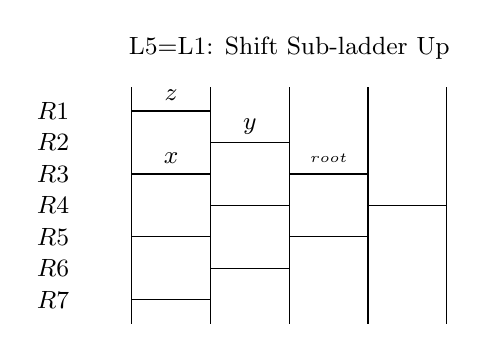
\begin{tikzpicture}
	 		\node at(2, 3.5){\small{L5=L1: Shift Sub-ladder Up}};
	 		\draw(0, 0) to (0, 3);
	 				\node at(.5, 2.9){\small{$z$}};
	 			\draw(0, 2.7) to (1,2.7);
	 				\node at(.5, 2.1){\small{$x$}};

	 			\draw(0,1.9) to (1,1.9);
	 			\draw(0,1.1) to (1,1.1);
	 			\draw(0,0.3) to (1,0.3);
	 		\draw(1, 0) to (1, 3);
	 			\node at(1.5,2.5){\small{$y$}};
	 			\draw(1,2.3) to (2,2.3);
	 			\draw(1,1.5) to (2,1.5);
	 			\draw(1,0.7) to (2,0.7);
	 		\draw(2, 0) to (2, 3);
	 			\node at(2.5, 2.1){\tiny{$root$}};
	 			\draw(2,1.9) to (3,1.9);
	 			\draw(2,1.1) to (3,1.1);
	 		\draw(3, 0) to (3, 3);
	 			\draw(3,1.5) to (4,1.5);
	 		\draw(4, 0) to (4, 3);

	 		\node at(-1, 2.7){\small{$R1$}};
	 		\node at(-1, 2.3){\small{$R2$}};
	 		\node at(-1, 1.9){\small{$R3$}};
	 		\node at(-1, 1.5){\small{$R4$}};
	 		\node at(-1, 1.1){\small{$R5$}};
	 		\node at(-1, .7){\small{$R6$}};
	 		\node at(-1, .3){\small{$R7$}};

		
	 	\end{tikzpicture}
	 \end{minipage}
	 \end{center}
	\caption{$x,y,z$ to be locally swapped. $root$ is the root of the sub-ladder.}
	\label{Fig:SwapAndShift}
\end{figure}

\begin{lemma}[h]
	The time complexity for performing a local swap operation is $CAT$, constant amortized time, per bar. 
\end{lemma}
\begin{proof}
	In the {\sc LeftSwap} and {\sc RightSwap} algorithms, calculating the row and column for $x,y$ and $z$ 
	along with the target row and column to swap each of these bars to is done in $O(1)$ time.
	In the algorithm {\sc ShiftSubLadder}, each recursive call swaps one or two bars. The row and 
	column for any given bar to be swapped is calculated in $O(1)$ time and the target row 
	and column for any given bar is calculated in $O(1)$ time.
\end{proof}

In concluding the section on the enumeration problem, we have analyzed the original paper along with 
making additions to the algorithm {\sc FindAllChildren} by providing four essential algorithms 
for the completion of {\sc FindAllChildren}. The algorithms are {\sc CreateRoot}, {\sc RightSwap},
{\sc LeftSwap} and {\sc ShiftSubLadder}. In concert, these five algorithms solve the enumeration 
problem which lists $OptL\{\pi\}$ in $O(1)$ time per ladder. 

